\documentclass[aspectratio=169]{beamer}



\mode<presentation>
{
 \usetheme[reversetitle,notitle,noauthor]{Wien}
%    \usetheme[noauthor]{Wien}
}

\usepackage{url}
\usepackage{graphicx}
\graphicspath{{./}{./Figures/}}

\usepackage{appendixnumberbeamer}
\usepackage{algorithm2e}
\usepackage{float}
\usepackage{tikz}
\usetikzlibrary{arrows.meta,positioning}
\usetikzlibrary{positioning}
\usetikzlibrary{overlay-beamer-styles}

\tikzset{onslide/.code args={<#1>#2}{%
  \only<#1>{\pgfkeysalso{#2}} % \pgfkeysalso doesn't change the path
}}
\tikzset{temporal/.code args={<#1>#2#3#4}{%
  \temporal<#1>{\pgfkeysalso{#2}}{\pgfkeysalso{#3}}{\pgfkeysalso{#4}} % \pgfkeysalso doesn't change the path
}}

\tikzstyle{highlight}=[red,ultra thick]

% To avoid a warning from the hyperref package:
\pdfstringdefDisableCommands{%
    \def\translate{}%
}

% To make sure, that the footnote is placed above and outside the
% footline (but it only works for one footnote per frame):
%
% \addtobeamertemplate{footnote}{}{\vspace{4ex}}

%%%%%%%%%%%%%%%%%%%%%%%%%%%%%%%%%%%%%%%%%%%%%%%%%%%%%%%%%%%%%%%%%%%%%%%%%%%%%
%%%%%%%%%%%%%%%%%%%%%%%%%%%%%%%%%%%%%%%%%%%%%%%%%%%%%%%%%%%%%%%%%%%%%%%%%%%%%
\title[Zelluläre Automaten]{Design und Analyse eines Spiels \newline mithilfe von Zellulären Automaten}


\subtitle{Bachelorarbeit aus Diskreter Mathematik}

\author[C. Göth]{Christian Göth}

\institute[TU Wien]{TU Wien, Vienna, Austria}

\date{21. Juni 2021}

% Hier befinden sich Pakete, die wir beinahe immer benutzen ...

\usepackage[utf8]{inputenc}

% Sprach-Paket:
\usepackage[ngerman]{babel}

% damit's nicht so, wie beim Grill aussieht:
\usepackage{fullpage}

% Mathematik:
\usepackage{amsmath, amssymb, amsfonts, amsthm}
\usepackage{bbm}
\usepackage{mathtools, mathdots}

% Makros mit mehereren Default-Argumenten:
\usepackage{twoopt}

% Anführungszeichen (Makro \Quote{}):
\usepackage{babel}

% if's für Makros:
\usepackage{xifthen}
\usepackage{etoolbox}

% tikz ist kein Zeichenprogramm (doch!):
\usepackage{tikz}

% bessere Aufzählungen:
\usepackage{enumitem}

% (bessere) Umgebung für Bilder:
\usepackage{graphicx, subfig, float}

% Umgebung für Code:
\usepackage{listings}

% Farben:
\usepackage{xcolor}

% Umgebung für "plain text":
\usepackage{verbatim}

% Umgebung für mehrerer Spalten:
\usepackage{multicol}

% "nette" Brüche
\usepackage{nicefrac}

% Spaltentypen verschiedener Dicke
\usepackage{tabularx}
\usepackage{makecell}

% Für Vektoren
\usepackage{esvect}

% (Web-)Links
\usepackage{hyperref}

% Zitieren & Literatur-Verzeichnis
\usepackage[style = authoryear]{biblatex}
\usepackage{csquotes}

% so ähnlich wie mathbb
%\usepackage{mathds}

% Keine Ahnung, was das macht ...
\usepackage{booktabs}
\usepackage{ngerman}
\usepackage{placeins}

% special letters:

\newcommand{\N}{\mathbb{N}}
\newcommand{\Z}{\mathbb{Z}}
\newcommand{\Q}{\mathbb{Q}}
\newcommand{\R}{\mathbb{R}}
\newcommand{\C}{\mathbb{C}}
\newcommand{\K}{\mathbb{K}}
\newcommand{\T}{\mathbb{T}}
\newcommand{\E}{\mathbb{E}}
\newcommand{\V}{\mathbb{V}}
\renewcommand{\S}{\mathbb{S}}
\renewcommand{\P}{\mathbb{P}}
\newcommand{\1}{\mathbbm{1}}

% quantors:

\newcommand{\Forall}{\forall \,}
\newcommand{\Exists}{\exists \,}
\newcommand{\ExistsOnlyOne}{\exists! \,}
\newcommand{\nExists}{\nexists \,}
\newcommand{\ForAlmostAll}{\forall^\infty \,}

% MISC symbols:

\newcommand{\landau}{{\scriptstyle \mathcal{O}}}
\newcommand{\Landau}{\mathcal{O}}


\newcommand{\eps}{\mathrm{eps}}

% graphics in a box:

\newcommandtwoopt
{\includegraphicsboxed}[3][][]
{
  \begin{figure}[!h]
    \begin{boxedin}
      \ifthenelse{\isempty{#1}}
      {
        \begin{center}
          \includegraphics[width = 0.75 \textwidth]{#3}
          \label{fig:#2}
        \end{center}
      }{
        \begin{center}
          \includegraphics[width = 0.75 \textwidth]{#3}
          \caption{#1}
          \label{fig:#2}
        \end{center}
      }
    \end{boxedin}
  \end{figure}
}

% braces:

\newcommand{\pbraces}[1]{{\left  ( #1 \right  )}}
\newcommand{\bbraces}[1]{{\left  [ #1 \right  ]}}
\newcommand{\Bbraces}[1]{{\left \{ #1 \right \}}}
\newcommand{\vbraces}[1]{{\left  | #1 \right  |}}
\newcommand{\Vbraces}[1]{{\left \| #1 \right \|}}
\newcommand{\abraces}[1]{{\left \langle #1 \right \rangle}}
\newcommand{\round}[1]{\bbraces{#1}}

\newcommand
{\floorbraces}[1]
{{\left \lfloor #1 \right \rfloor}}

\newcommand
{\ceilbraces} [1]
{{\left \lceil  #1 \right \rceil }}

% special functions:

\newcommand{\norm}  [2][]{\Vbraces{#2}_{#1}}
\newcommand{\diam}  [2][]{\mathrm{diam}_{#1} \: #2}
\newcommand{\diag}  [1]{\mathrm{diag} \: #1}
\newcommand{\dist}  [1]{\mathrm{dist} \: #1}
\newcommand{\mean}  [1]{\mathrm{mean} \: #1}
\newcommand{\erf}   [1]{\mathrm{erf} \: #1}
\newcommand{\id}    [1]{\mathrm{id} \: #1}
\newcommand{\sgn}   [1]{\mathrm{sgn} \: #1}
\newcommand{\supp}  [1]{\mathrm{supp} \: #1}
\newcommand{\arsinh}[1]{\mathrm{arsinh} \: #1}
\newcommand{\arcosh}[1]{\mathrm{arcosh} \: #1}
\newcommand{\artanh}[1]{\mathrm{artanh} \: #1}
\newcommand{\card}  [1]{\mathrm{card} \: #1}
\newcommand{\Span}  [1]{\mathrm{span} \: #1}
\newcommand{\Aut}   [1]{\mathrm{Aut} \: #1}
\newcommand{\End}   [1]{\mathrm{End} \: #1}
\newcommand{\ggT}   [1]{\mathrm{ggT} \: #1}
\newcommand{\kgV}   [1]{\mathrm{kgV} \: #1}
\newcommand{\ord}   [1]{\mathrm{ord} \: #1}
\newcommand{\grad}  [1]{\mathrm{grad} \: #1}
\newcommand{\ran}   [1]{\mathrm{ran} \: #1}
\newcommand{\graph} [1]{\mathrm{graph} \: #1}
\newcommand{\Inv}   [1]{\mathrm{Inv} \: #1}
\newcommand{\pv}    [1]{\mathrm{pv} \: #1}
\newcommand{\GL}    [1]{\mathrm{GL} \: #1}
\newcommand{\Mod}{\mathrm{Mod} \:}
\newcommand{\Th}{\mathrm{Th} \:}
\newcommand{\Char}{\mathrm{char}}
\newcommand{\At}{\mathrm{At}}
\newcommand{\Ob}{\mathrm{Ob}}
\newcommand{\Hom}{\mathrm{Hom}}
\newcommand{\orthogonal}[3][]{#2 ~\bot_{#1}~ #3}
\newcommand{\Rang}{\mathrm{Rang}}
\newcommand{\NIL}{\mathrm{NIL}}
\newcommand{\Res}{\mathrm{Res}}
\newcommand{\lxor}{\dot \lor}
\newcommand{\Div}{\mathrm{div} \:}
\newcommand{\meas}{\mathrm{meas} \:}

% fractions:

\newcommand{\Frac}[2]{\frac{1}{#1} \pbraces{#2}}
\newcommand{\nfrac}[2]{\nicefrac{#1}{#2}}

% derivatives & integrals:

\newcommandtwoopt
{\Int}[4][][]
{\int_{#1}^{#2} #3 ~\mathrm{d} #4}

\newcommandtwoopt
{\derivative}[3][][]
{
  \frac
  {\mathrm{d}^{#1} #2}
  {\mathrm{d} #3^{#1}}
}

\newcommandtwoopt
{\pderivative}[3][][]
{
  \frac
  {\partial^{#1} #2}
  {\partial #3^{#1}}
}

\newcommand
{\primeprime}
{{\prime \prime}}

\newcommand
{\primeprimeprime}
{{\prime \prime \prime}}

% Text:

\newcommand{\Quote}[1]{\glqq #1\grqq{}}
\newcommand{\Text}[1]{{\text{#1}}}
\newcommand{\fastueberall}{\text{f.ü.}}
\newcommand{\fastsicher}{\text{f.s.}}

\theoremstyle{definition}

% unnumbered theorems
\newtheorem*{theorem*}    {Satz}
\newtheorem*{lemma*}      {Lemma}
\newtheorem*{corollary*}  {Korollar}
\newtheorem*{proposition*}{Proposition}
\newtheorem*{remark*}     {Bemerkung}
\newtheorem*{definition*} {Definition}
\newtheorem*{example*}    {Beispiel}
\newtheorem*{problem*}    {Problem}
\newtheorem*{algorithmus*}    {Algorithmus}
\newtheorem*{algorithmen*}    {Weiterführende Algorithmen}
\newtheorem*{anwendungen*}    {Anwendungen}

\renewcommand{\figurename}{Abbildung}
\renewcommand{\tablename} {Tabelle}


\begin{document}

\begin{frame}
    \titlepage
\end{frame}

%%%%%%%%%%%%%%%%%%%%%%%%%%%%%%%%%%%%%%%%%%%%%%%%%%%%%%%%%%%%%%%%%%%%%%%%%%%%%
%%%%%%%%%%%%%%%%%%%%%%%%%%%%%%%%%%%%%%%%%%%%%%%%%%%%%%%%%%%%%%%%%%%%%%%%%%%%%
%%%%%%%%%%%%%%%%%%%%%%%%%%%%%%%%%%%%%%%%%%%%%%%%%%%%%%%%%%%%%%%%%%%%%%%%%%%%%


  \begin{frame}{Wiederholung 1/2}
    \begin{block}{Definitionen (Bestandteile eines ZA)}
      \begin{itemize}
        \item \textit{Zellularraum} $\mathbb{Z}^{d}$: $d$-dimensionales unendliches Gitter
        \item \textit{Zustandsmenge} $S$: endliche Menge
        \item \textit{Nachbarschaft}: Vektor $N = (y_1,y_2,\dots,y_n)$ aus $n$ paarweise verschiedenen Elementen
        \item \textit{Lokale Update-Regel} $f: S^n \to S$
      \end{itemize}
    \end{block}

    \pause

    \begin{definition*}
      \begin{itemize}
        \item \textit{Konfiguration}: Abbildung $c: \mathbb{Z}^{d} \to S$
        \item Die Menge $S^{\mathbb{Z}^{d}}$ aller Konfigurationen heißt $\mathcal{C}(d,S) = \mathcal{C}$
      \end{itemize}
    \end{definition*}
  \end{frame}


  \begin{frame}{Eigenschaften des Spiels 1/3}
    \begin{block}{Zustandsmenge}
      Jeder Zustand besteht aus $4$ Komponenten $(\uparrow, \rightarrow, \downarrow, \leftarrow)$, die einer (theoretischen) Mehrfach-Belegung entsprechen:
      \begin{align*}
        & S := \{0,1\}^4 \cup \{0,2,3\}^{4} \\
        \Rightarrow & |S| = 2^4 + 3^4 -1 = 96
      \end{align*}

    \end{block}

    \pause

    \begin{block}{Nachbarschaft ($n=9$)}
      \begin{figure}[H]
          \centering
          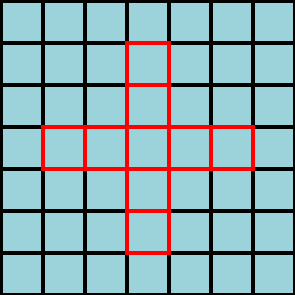
\includegraphics[width = 0.2 \textheight]{neighborhood.png}
      \end{figure}

    \end{block}
  \end{frame}


  \begin{frame}{Eigenschaften des Spiels 2/3}
    \begin{block}{Lokale Update-Regel}
      Sehr komplex ($f: S^n \to S$ mit $|S^n| = 96^9$) und diverse Fallunterscheidungen. \\
      Daher nur zwei Beispiele.
    \end{block}

    \pause

    \begin{multicols*}{3}

      \begin{figure}[H]
        \centering
        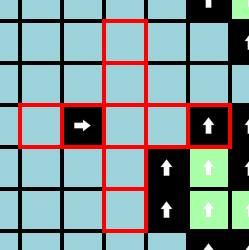
\includegraphics[width = 0.39 \textheight]{example1n_1.png}
      \end{figure}

      \vfill\null

      \pause

      \begin{figure}[H]
        \centering
        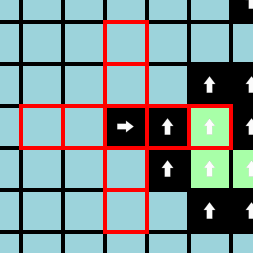
\includegraphics[width = 0.39 \textheight]{example1n_2.png}
      \end{figure}

      \vfill\null

      \pause


      \begin{figure}[H]
        \centering
        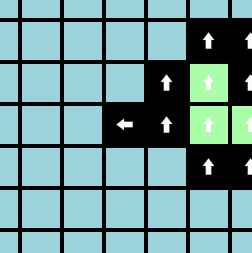
\includegraphics[width = 0.39 \textheight]{example1_3.png}
      \end{figure}

    \end{multicols*}

  \end{frame}

  \begin{frame}{Eigenschaften des Spiels 3/3}
    \begin{block}{Lokale Update-Regel}
      Sehr komplex ($f: S^n \to S$ mit $|S^n| = 96^9$) und diverse Fallunterscheidungen. \\
      Daher nur zwei Beispiele.
    \end{block}

    \begin{multicols*}{3}

      \begin{figure}[H]
        \centering
        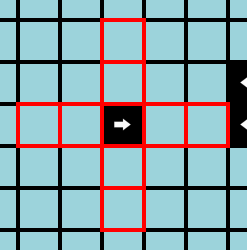
\includegraphics[width = 0.39 \textheight]{example2n_1.png}
      \end{figure}

      \vfill\null

      \pause

      \begin{figure}[H]
        \centering
        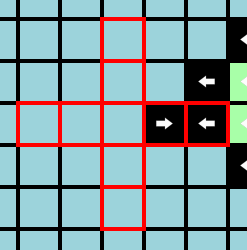
\includegraphics[width = 0.39 \textheight]{example2n_2.png}
      \end{figure}

      \vfill\null

      \pause


      \begin{figure}[H]
        \centering
        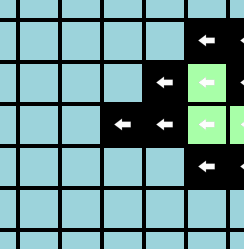
\includegraphics[width = 0.39 \textheight]{example2_3.png}
      \end{figure}

    \end{multicols*}

  \end{frame}



  \begin{frame}{Eigenschaften des Spiels (Ausblick)}
    Erweiterung von $S, N$ und $f$ bei Eingreifen des\slash der Spieler\textunderscore in.

    \vfill\null

    \begin{multicols*}{2}

      \begin{figure}[H]
        \centering
        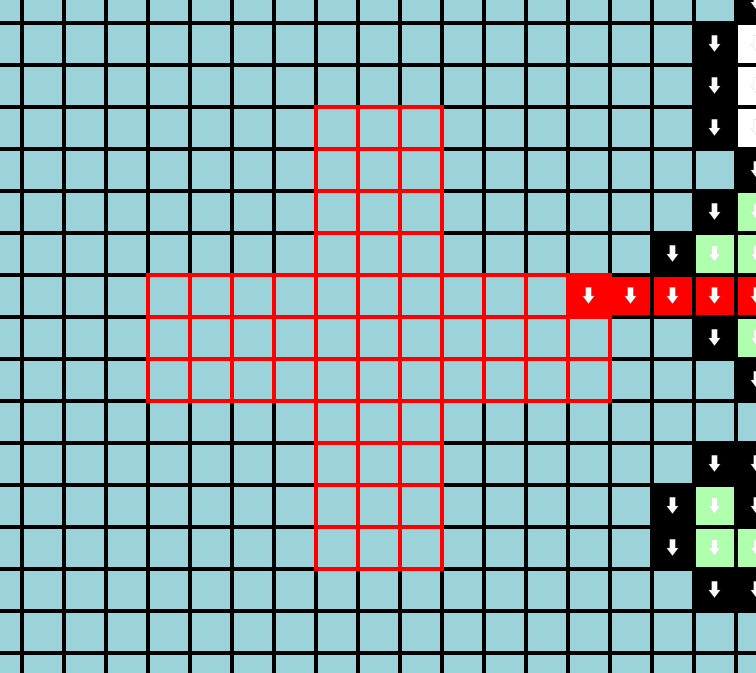
\includegraphics[width = 0.5 \textheight]{example3n_1.png}
      \end{figure}


      \pause

      \begin{figure}[H]
        \centering
        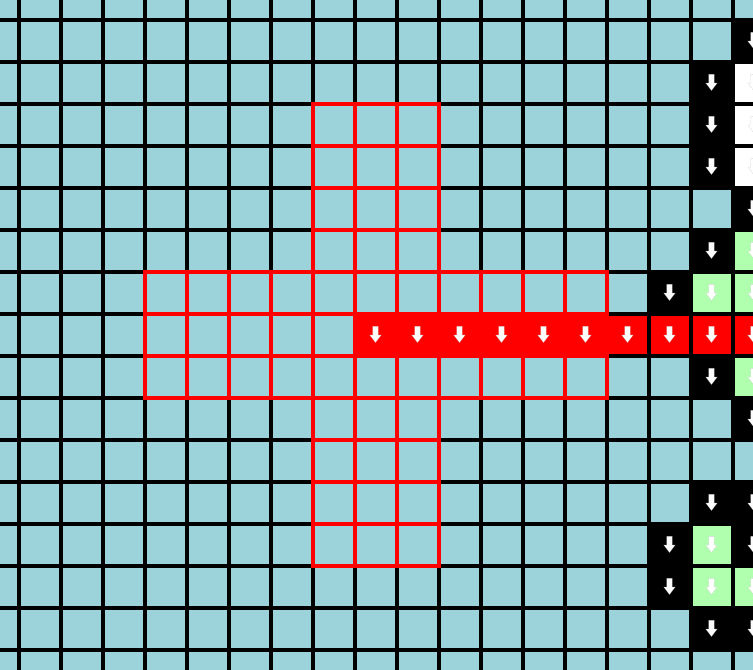
\includegraphics[width = 0.5 \textheight]{example3n_2.png}
      \end{figure}

    \end{multicols*}

  \end{frame}

  \begin{frame}{Wiederholung 2/2}
    \begin{definition*}
      Wir identifizieren einen zellulären Automaten $(S,N,f)$ mit seiner \textit{Globalen Überführungsfunktion} $G: \mathcal{C} \to \mathcal{C}$ und sprechen vom ZA $G$.
    \end{definition*}

    \pause

    \begin{definition*}
      Ein ZA $G$ heißt bijektiv, falls $G$ als Funktion bijektiv ist.
    \end{definition*}

    \begin{definition*}
      Ein ZA $G$ heißt reversibel, falls ein ZA $H$ existiert mit $G \circ H = H \circ G = id$.
    \end{definition*}
  \end{frame}


  \begin{frame}{Definitionen}
    \begin{definition*}
      Auf der Menge $\mathcal{C} = S^{\mathbb{Z}^d}$ der Konfigurationen definieren wir nun eine Metrik. Für $c, e \in \mathcal{C}$ sei
      \begin{align*}
        d(c, e) = \begin{cases}
          0, & c = e \\
          2^{- \min \{ \|x\|_\infty: c(x) \neq e(x)\} }& \, c \neq e
        \end{cases}
      \end{align*}
    \end{definition*}

    \pause

    \begin{remark*}
      Es ist $d$ tatsächlich eine Metrik. Die induzierte Topologie entspricht der Produkt- topologie der diskreten Topologie von $S$ und macht $\mathcal{C}$ zu einem kompakten Raum.
    \end{remark*}

    \pause

    \begin{definition*}
      Für $y \in \mathbb{Z}^d$ definieren wir den ZA $\tau_{y} = (S, (-y), id)$ und nennen ihn \textit{Translation} um den Vektor $y$.
    \end{definition*}

  \end{frame}

  \begin{frame}{Curtis-Hedlund-Lyndon Theorem}
    \begin{theorem*}[Curtis-Hedlund-Lyndon]
      Eine Funktion $G: S^{\mathcal{Z}^d} \to S^{\mathcal{Z}^d}$ ist die Globale Überführungsfunktion eines ZA genau dann, wenn $G$ stetig ist und mit Translationen kommutiert.
    \end{theorem*}

    \pause

    \begin{corollary*}
      Ein ZA $G$ ist reversibel genau dann, wenn er bijektiv ist.
    \end{corollary*}

    \begin{proof}
      Definitionsgemäß folgt aus der Reversibilität die Bijektivität.
      Sie $G$ ein bijektiver ZA. Die Inverse $G^{-1}$ einer stetigen Bijektion zwischen zwei kompakten metrischen Räumen ist wieder stetig. Offensichtlich kommutiert $G^{-1}$ mit Translationen. Somit ist $G^{-1}$ die Funktion eines ZA.
    \end{proof}
  \end{frame}


  \begin{frame}{Injektivität in Zellulären Automaten}
    \begin{corollary*}
      Ein ZA $G$ ist reversibel genau dann, wenn er bijektiv ist.
    \end{corollary*}

    \pause

    \begin{theorem*}[Garden-of-Eden/ Moore and Myhill]
      Ein ZA $G$ ist surjektiv genau dann, wenn die Einschränkung auf endliche Konfigurationen $G_F$ injektiv ist.
    \end{theorem*}

    \pause

    Es gilt also für Zelluläre Automaten:
    \begin{align*}
      \text{Injektivität} \Leftrightarrow \text{Reversibilität}.
    \end{align*}
  \end{frame}


  \begin{frame}{\sout{Injektivität}}

    \begin{multicols*}{5}

      \onslide<1->\begin{figure}[H]
        \centering
        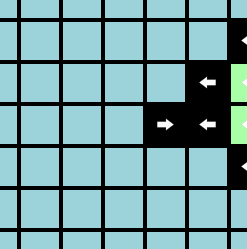
\includegraphics[width = 0.35 \textheight]{example2_2.png}
      \end{figure}

      \vfill\null

      \onslide<2->\centering{\Huge $\rightarrow$ \par}

      \vfill\null

      \onslide<2->\begin{figure}[H]
        \centering
        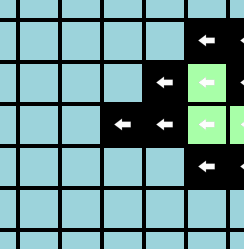
\includegraphics[width = 0.35 \textheight]{example2_3.png}
      \end{figure}

      \vfill\null



      \onslide<3->\centering{\Huge $\leftarrow$ \par}
      \vfill\null

      \onslide<3->\begin{figure}[H]
        \centering
        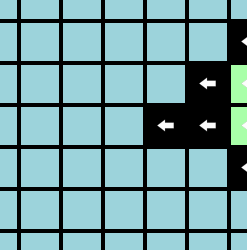
\includegraphics[width = 0.35 \textheight]{example4_2.png}
      \end{figure}

    \end{multicols*}
  \end{frame}


  \begin{frame}{Garden of Eden-Konfigurationen}
    \begin{figure}[H]
      \centering
      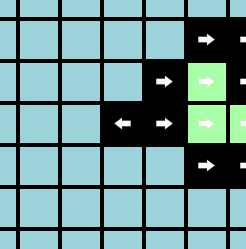
\includegraphics[width = 0.55 \textheight]{example5.png}
    \end{figure}
  \end{frame}


  \begin{frame}{}
    \begin{block}{}

      {
          \centering
          \huge
          Bei Interesse am Spiel gerne melden!
      }

    \end{block}

  \end{frame}


\end{document}


%%% Local Variables:
%%% mode: latex
%%% TeX-master: t
%%% End:
